\documentclass[sn-mathphys-num]{sn-jnl}
\usepackage{graphicx}%
\usepackage{multirow}%
\usepackage{amsmath,amssymb,amsfonts}%
\usepackage{amsthm}%
\usepackage{mathrsfs}%
\usepackage[title]{appendix}%
\usepackage{xcolor}%
\usepackage{textcomp}%
\usepackage{manyfoot}%
\usepackage{booktabs}%
\usepackage{algorithm}%
\usepackage{algorithmicx}%
\usepackage{algpseudocode}%
\usepackage{listings}%
\theoremstyle{thmstyleone}
\newtheorem{theorem}{Theorem}
\newtheorem{proposition}[theorem]{Proposition}
\theoremstyle{thmstyletwo}%
\newtheorem{example}{Example}%
\newtheorem{remark}{Remark}%

\theoremstyle{thmstylethree}%
\newtheorem{definition}{Definition}%

\raggedbottom

\bibliographystyle{elsarticle-num}

\usepackage{array}
\usepackage{tabularx}

\begin{document}

\title[Article Title]{SNR-Responsive Communication: Turbo Codes and BCH in a Dynamic HARQ Scheme for Enhanced Efficiency}

\author[1]{\fnm{C. } \sur{Gnana Jyothi}}\email{chinthagnanajyothi.221cs118@nitk.edu.in}
\author[2]{\fnm{P. } \sur{Chandana Sai Sri Hasitha}}\email{prathapachandanasaisrihasitha.221cs139@nitk.edu.in}
\author[3]{\fnm{N. } \sur{Yaswanth}}\email{namburiyaswanth.221cs232@nitk.edu.in}
\author*[4]{\fnm{B. R.} \sur{Chandavarkar}}\email{brc@nitk.edu.in}
	
\affil*[1]{\centering \orgdiv{Department of Computer Science and Engineering}, \\ \orgname{National Institute of Technology Karnataka, Surathkal}, \\ \orgaddress{\city{Mangaluru-575025}, \state{Karnataka}, \country{India}}}

\abstract{Wireless communication systems face many challenges due to fluctuating channel conditions resulting in variable error rates and demands robust error management tactics. Traditional Automatic Repeat Request (ARQ) methods suffer from high communication overhead and latency and are inefficient in handling retransmissions. Although traditional Hybrid Automatic Repeat Request (HARQ) is effective, its widespread use is limited by high implementation costs. This underscores the need for adaptive systems that dynamically respond to changing channel conditions based on Signal-to-Noise ratio (SNR). This paper proposes the Dynamic HARQ (D-HARQ), which switches between ARQ, HARQ with Bose-Chaudhuri-Hocquenghem (BCH) codes, and HARQ with turbo codes based on channel conditions during the transmission. Further, this paper incorporates a selective soft-combining technique by estimating the receiver end's signal-to-noise ratio (SNR). The main goal is to achieve the maximum possible throughput even at very low SNR values while maintaining optimal complexity.}

\keywords{Adaptive HARQ, SNR estimation, Turbo codes, BCH codes, Selective soft combining, Error correction, Throughput optimization}

\maketitle

\section{Introduction}\label{s1}

Error control mechanisms play a crucial role in reliable data transmission. Ensures retransmission of data packets that are found to be erroneous or lost during the transmission. The end-to-end transfer of data from one application to another involves several steps, each subject to errors along the way \cite{r5}. Due to the necessity of numerous retransmissions, standard Automatic Repeat Request (ARQ) schemes do not adequately correct all errors. Thus, this paper uses Hybrid ARQ (HARQ), which integrates ARQ with Forward Error Correction (FEC) \cite{r14, r13} for its improved efficiency in this context. However, this system may not be necessary under good channel conditions. To address this issue, this paper is developing a multifunctional approach that adjusts to the varying needs of different channel conditions.

\subsection{Go-Back-N (GBN) Scheme } \label{s1.1}

GBN scheme \cite{r26} is one of the Pure ARQ methods. In this scheme, the sender sends a sequence of frames without waiting for acknowledgment until a specified window size is reached. If errors are detected or the packet is lost, then negative acknowledgment (NACK) \cite{r12}  is sent, and the sender resends all frames starting from the last acknowledged frame. Figure \ref{fig:1} illustrates the GBN scheme, where the sender (transmitter) transmits a sequence of frames (M1, M2, M3, etc.) to the receiver. The receiver acknowledges the correctly received frames with ACK messages (ACK1, ACK2, etc.). If a frame is lost or corrupted, the receiver sends a negative acknowledgment (NACK4 in the figure), prompting the sender to retransmit all frames starting from the lost frame (M4 in this case). This scheme does not require a storage buffer on the receiver side. GBN guarantees data integrity and reduces network congestion.

\begin{figure}[H]
    \centering
    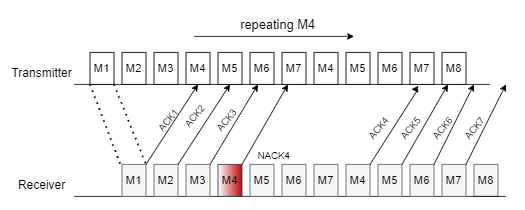
\includegraphics[width=0.8\textwidth]{gbn.png}
    \caption{Go Back-N (GBN) scheme \cite{r12}}
    \label{fig:1}
\end{figure}

\subsection{Hybrid ARQ } \label{s1.2}

The Hybrid ARQ \cite{r1, r50} is the ARQ concatenated with FEC. This facilitates error correction during transmission, minimizing the likelihood of receiving additional errors. Retransmission occurs when packet errors remain uncorrected. HARQ mainly has two basic schemes: Hybrid ARQ Type I, which has adaptive coding rates and extra error-correcting codes to minimize retransmissions while maintaining data integrity. The Hybrid ARQ Type II uses redundancy to improve the error correction capabilities later. These approaches guarantee robust data transmission, optimization of throughput, and reliable communication.
 
\subsection{Turbo Codes}  \label{s1.3}

Turbo codes \cite{r22} are part of error correction codes that employ parallel concatenated convolutional codes to achieve remarkably efficient error correction. They are most commonly used in 3G/4G mobile communications (e.g. LTE) and in satellite communications, where there is a high demand for reliable information transfer. Turbo codes offer superior performance in noisy channels by iteratively decoding received signals. They take advantage of the redundancy provided by multiple convolutional codes in parallel. This iterative decoding process allows turbo codes to approach the Shannon limit. In Turbo codes, the code rate refers to the ratio of information bits to the total number of transmitted bits. The natural coding rate of a turbo code is R = 1/3 (three output bits for one input bit). 

\begin{figure}[H]
    \centering
    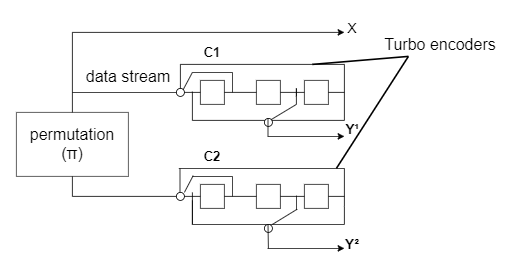
\includegraphics[width=0.8\textwidth]{Turbo_diagram.png}
    \caption{A classical Turbo code \cite{r25}}
    \label{fig:12}
\end{figure}

Figure \ref{fig:12} depicts a classical Turbo Code structure, which consists of the parallel concatenation of two binary convolutional encoders, C1 and C2, separated by a permutation (interleaver) block labeled $\pi$. The input data stream X is fed directly into the first encoder C1, producing the systematic output y1. The same input data X is also passed through the permutation block ($\pi$), which rearranges or interleaves the order of the data bits before feeding them into the second encoder C2, generating the parity output y2. Therefore, the outputs of the Turbo Code encoder are y1, an exact copy of the input data X (systematic output of C1), and y2, the parity output of C2, after interleaving the input data. The systematic and parity outputs (y1 and y2) are then transmitted. The key idea behind the Turbo Code structure is that interleaved introduces redundancy and randomizes the input data, allowing the parallel encoders to provide robust error correction capabilities when decoding at the receiver end. Despite the high error-correcting capability, they are quite complex to implement.

\subsection{Soft Combining} \label{s1.4}

Soft combining \cite{r15} is a technique in which an erroneous packet received is stored in a buffer rather than discarded. Two independently uncorrectable erroneous packets can be correctly decoded by using the useful information obtained from their combination. This scheme has two main methods: chase combining and Incremental Redundancy (IR).In chase combining, every retransmitted packet is the same as the previous one. With maximum ratio combining, the receiver combines the newly received bits with the previously received ones, including any errors. This increases the total signal energy for each retransmission, effectively improving the $Eb/N_0$ ratio. In incremental redundancy, different redundancy bits are obtained by puncturing the encoder output, thus adding additional information to each retransmission.

\begin{figure}[H]
    \centering
    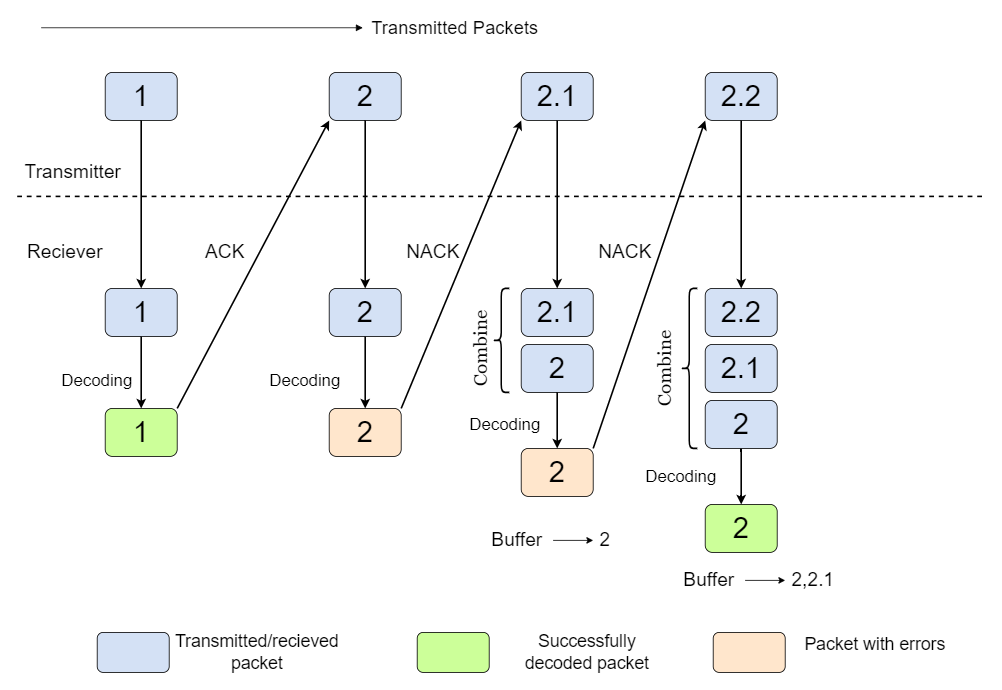
\includegraphics[width=0.8\textwidth]{Soft_Combining_3.png}
    \caption{Illustration of Soft combining with HARQ  \cite{r23}}
    \label{fig:10}
\end{figure}

Figure \ref{fig:10} illustrates the concept of soft combining with HARQ in a communication system. The transmitter sends packets, which are received and decoded by the receiver. An ACK is returned to the transmitter if a packet is correctly decoded. A NACK is sent and stored in a buffer if errors occur in the received packet. The transmitter then resends the erroneous packet and the receiver combines (soft combining) the previously stored erroneous packet with the newly received packet to improve the decoding process. This combining process is repeated for subsequent NACKs and retransmissions, with the buffer storing the combined packets (e.g., 2, 2.1, 2.2.1). The soft combining technique improves the reliability of data transmission by utilizing the information from previous erroneous transmissions, leading to improved error correction and overall system performance.

Several existing error-correcting mechanisms are easy to implement but do not offer strong error-correction capabilities, while others are complex but provide robust error-correction. Therefore, the choice of FEC \cite{r14} should be based on the channel conditions. Many existing approaches involve repeated retransmissions because they discard corrupted packets instead of utilizing them. These schemes are of great significance in DVB (Digital Video Broadcasting), storage systems (such as CDs, DVDs, and flash memory) and satellite communication systems \cite{r18}.

This paper improves system efficiency by dynamically switching among ARQ, HARQ with Turbo Codes, and HARQ with BCH codes based on fluctuating SNR values. Furthermore, it introduces a novel mechanism for selective soft combining packets at the receiver end based on current channel conditions. This approach minimizes retransmissions by using corrupted packets instead of discarding them.This method significantly enhances throughput across all scenarios by selecting the appropriate scheme at each transmission stage.

The rest of the paper is organized as follows: Section \ref{s2} covers the literature survey, while Section \ref{s3} explains the design and implementation of the proposed solution. Section \ref{s4} presents the simulation results, analysis, and comparisons with existing methods. Finally, Section \ref{s5} concludes with future directions and references.

\section{Literature survey} \label{s2}

This section discusses the various adaptive HARQ schemes followed by their advantages and drawbacks. Firstly, in Subsection \ref{s2.1}, the Adaptive HARQ with Reed-Solomon (RS) codes utilizes a straightforward approach based on consecutive ACKs and NACKs to dynamically switch between the HARQ and ARQ modes. Secondly, in Subsection \ref{s2.2}, the Adaptive HARQ with two RS codes proposes a three-stage adaptive approach, dividing high channel error rates into HARQ1 and HARQ2 states with different RS code rates to optimize error correction efficiency. Lastly, in Subsection \ref{s2.3}, the Adaptive HARQ with BCH codes dynamically switches between the HARQ1 and HARQ2 schemes based on estimated channel states and SNR thresholds, effectively addressing a wide range of channel conditions using hybrid BCH code schemes. 

\subsection{Adaptive HARQ with Reed-Solomon codes} \label{s2.1}

Peter Fidler et al. \cite{r6} introduced the adaptation rule that employs a straightforward approach based on counting consecutive acknowledgments (ACKs) and negative acknowledgments (NACKs) to dynamically switch between HARQ and ARQ modes, depending on the estimated channel state. As depicted in Figure \ref{fig:2}, the key component of this model is the threshold parameter (T), which sets a limit on consecutive ACKs required to transition from HARQ to ARQ mode. Once the number of consecutive ACKs exceeds this threshold, the system shifts to the less complex ARQ mode, signifying a stable channel condition. In contrast, detecting even a single NACK prompts an immediate switch back to HARQ mode, reflecting the need for enhanced error correction in response to channel degradation.

\begin{figure}[H]
    \centering
    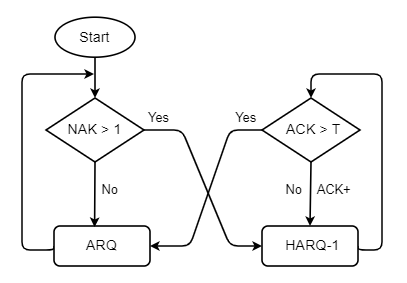
\includegraphics[width=0.6\textwidth]{rs.png}
    \caption{Adaptive HARQ using RS codes \cite{r6}}
    \label{fig:2}
\end{figure}

This schema offers several advantages. First, its adaptive system dynamics introduce an asymmetrical strategy that swiftly transitions to the HARQ mode upon detecting a noisy channel.This dynamic approach requires a threshold of positive acknowledgments to switch back to ARQ mode, ensuring that the system remains robust and responsive to real-time channel conditions. This schema has several disadvantages, such as limited adaptability with only two states, which restricts the system adjustment to high fluctuations in channel quality. This has limited scalability for complex network environments.

\subsection{Adaptive HARQ with two RS codes} \label{s2.2}

Michal M. et al. \cite{r8} proposed a three-stage adaptive ARQ/HARQ1/HARQ2 scheme. The number of states is increased compared to the previously discussed adaptive HARQ scheme, and relatively higher throughput for various channel bit error rates can be achieved. There are three operating modes: pure ARQ -Go Back -N \cite{r18}, HARQ1 with RS code (511, 383, 64), and HARQ2 with RS code (511, 255, 128). The transmitter follows the pure ARQ method for the state L of low channel error rate. The previously discussed high channel error rate is now divided into HARQ1 and HARQ2. Both states use RS code but with different code rates. 

\begin{figure}[H]
    \centering
    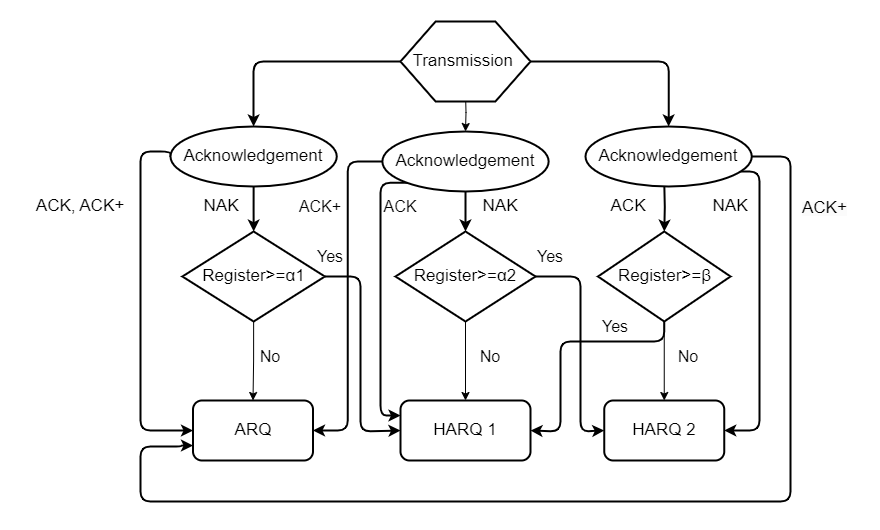
\includegraphics[width=0.9\textwidth]{two_rs.png}
    \caption{Dynamic Adaption of different HARQ schemes using two RS codes \cite{r8}}
    \label{fig:3}
\end{figure}

Figure \ref{fig:3} explains that the switching logic operates so that the transmitter manages the switch from ARQ to HARQ modes or HARQ1 to HARQ2. The receiver handles the switch from the HARQ modes to ARQ modes. These three confirmations are utilized in the proposal \cite{r8} as follows:
   \begin{itemize}
       \item ACK when the packet contains no errors (pure ARQ) or when the packet can be corrected by the RS code (HARQ1, HARQ2).
       \item NAK when the RS code cannot rectify the packet (HARQ1, HARQ2).
       \item  ACK+ when there is no error in the previous W packets.
   \end{itemize}

This paper brings several advantages firstly, it introduces a pioneering approach through a 3-stage proposal with a sliding window mechanism. Unlike conventional ARQ-HARQ methods with fewer stages, this multistage scheme offers flexibility and adaptability to diverse channel conditions. However, this approach does not handle a broader range of SNR values, optimize throughput, and minimize latency. This approach also has drawbacks, such as increased latency for real-time traffic and limited capability in correcting random errors due to its RS error-correcting code.

\subsection{Adaptive HARQ with BCH codes } \label{s2.3}

F. C. Kvetoslava Kotuliakova et al. \cite{r5} presented an improved adaptive ARQ-HARQ method \cite{r20} that uses BCH codes and is intended to improve the effectiveness of data transmission under varying channel conditions. This scheme dynamically modifies the transmission schemes in response to the measured bit error rate of the channel. Figure \ref{fig:4} shows an adaptive HARQ model that dynamically switches between the HARQ1 and HARQ2 schemes, which have different code rates, based on the estimated state of the channel and the SNR threshold. The process starts by estimating the state of the channel. If the SNR exceeds the threshold, it uses the GBN scheme, which is more efficient for good channel conditions. Otherwise, it checks if the channel is in a bad state (HARQ2). If so, it uses the HARQ2 scheme with a higher code rate, which is suitable for poor channel conditions to improve reliability. If the channel is not in a bad state, it uses the HARQ1 scheme with a medium code rate. The system smoothly switches to hybrid ARQ schemes as the error rate increases to moderate to high levels. 

\begin{figure}[H]
    \centering
    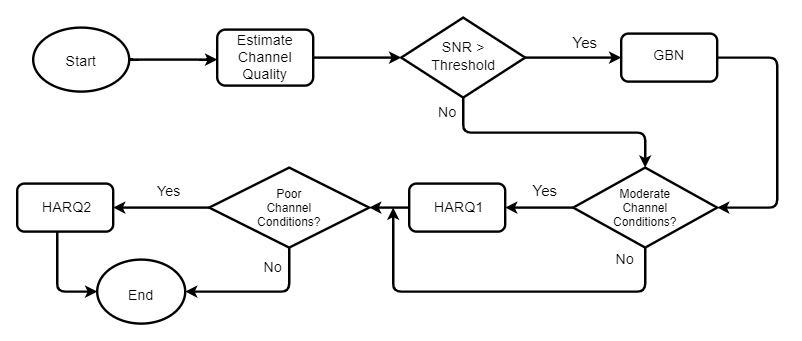
\includegraphics[width=0.9\textwidth]{bch_t.png}
    \caption{Adaptive HARQ using BCH codes \cite{r5}}
    \label{fig:4}
\end{figure}

These hybrid schemes combine two selected BCH codes to improve error correction performance in various channel conditions. The GBN \cite{r18} protocol is used in all modes for better performance, as discussed in Subsection \ref{s1.1}. This adaptive strategy shows great promise for establishing reliable and effective data communication in various difficult-to-manage channel conditions.

This scheme has various advantages, including dynamically altering parameters to adapt to changing network conditions and effectively controlling retransmissions; the scheme greatly reduces latency and improves system responsiveness. The disadvantage of this schema is that there are difficulties in maintaining effective data transmission under low SNR conditions. In such conditions, it has almost zero throughput.

\section{Design and Implementation of Dynamic HARQ (D-HARQ)} \label{s3}

This section of the paper discusses the design and implementation of the D-HARQ scheme to improve communication efficiency. Firstly, Subsection \ref{s3.2} provides insight into the throughput analysis for various schemes, including pure ARQ, HARQ with BCH, and turbo codes, elucidating their performance under varying channel conditions. Secondly, Subsection \ref{s3.3} outlines a dynamic switching scheme between HARQ modes and pure ARQ based on NACK/ACK counts and SNR thresholds. Third, Subsection \ref{s3.4} delves into the mechanism of HARQ with Turbo Codes, emphasizing error correction and throughput improvement in low SNR scenarios. Fourth, in Subsection \ref{s3.1}, discussing a robust SNR estimation algorithm based on the Error Vector Magnitude (EVM) analysis is crucial for the selective soft combining scheme. Lastly, Subsection \ref{s3.5} discusses decision-making for soft combining at the receiver end.

D-HARQ dynamically adapts to different schemes based on real-time fluctuations in SNR values. When SNR is very low, it switches to robust turbo codes with HARQ for error correction. In contrast, when the SNR is moderate to high, it employs HARQ with BCH codes of different code rates. In particular, when the SNR reaches an extremely high value, the scheme strategically switches back to pure ARQ to maintain simplicity. The scheme operates in four states: Pure ARQ with Go-back N, two enhanced BCH codes HARQ1(4599, 3447) and HARQ2(4599, 2295), and an optimal state using HARQ with Turbo codes.

\subsection{Throughput of different schemes} \label{s3.2}

The first stage of implementation is a calculation of the throughput of different schemes like Pure ARQ, HARQ with BCH code, and HARQ with turbo codes. If the transmitter follows pure ARQ with GBN scheme, then the throughput is given by Eq. \ref{6}. Due to error detection bits, this throughput is multiplied by the weight, i.e., the ratio of message symbols to the total number of symbols.

\begin{equation}\label{6} 
    \eta_{\text{L}} = \frac{1 - P_e}{1 + S \cdot P_e} \cdot \frac{N - CRC}{N} 
\end{equation} 

Here, $N$ is the length of the block and ${P}_e$ is the probability of the occurrence of an error in the packet in the pure ARQ method. ${P}_e$ depends on the channel bit error rate, burst errors, and block length. This is expressed in Eq. \ref{7}.
 
\begin{equation}\label{7} 
    P_e = 1 - (1 - P_b)^K
\end{equation}

Where ${P}_b$ is the bit error rate. CRC is the number of redundancy symbols added for error detection, and S is defined as the ratio between the acknowledgment time delay and the time of block transmission.

\begin{equation}\label{8}
     S = T_a / T_b
\end{equation}

${T}_a$ is the acknowledgment time delay, defined as the time delay from terminating block transmission to receiving and processing block acknowledgment, and ${T}_b$ is the block transmission time, b is no.of bits per each symbol.

\begin{equation}\label{9}
    b = \log_2(N+1)
\end{equation}

If the transmission is in the HARQ scheme, the throughput will be as follows :

\begin{equation}\label{10}
    \eta_H = \frac{K}{N} \times \frac{1 - \sum_{i=t+1}^{N} \binom{N}{i} P_s^i (1-P_s)^{N-i}}{1 + S \cdot \sum_{i=t+1}^{N} \binom{N}{i} P_s^i (1-P_s)^{N-i}}
\end{equation}

Where ${P}_s$ is the probability that the symbol has an error and is calculated as below: 
 
\begin{equation}\label{11}
    P_s = 1 - (1 - P_b)^b
\end{equation}

If the transmitter chooses to use turbo codes with a code rate of 1/3 as the error correction scheme, the throughput is determined by the following calculation.

 \begin{equation}
T_{\text{hr}} = \left(\frac{R_{c}}{T_{r}}\right) \cdot \left(\frac{k}{k + n_{p}}\right)
\end{equation}

Where k/(k + ${n}_p$) is the fractional throughput loss due to additional parity bits added to detect errors, where k is the number of information bits and ${n}_p$ is the number of parity bits. ${R}_c$ denotes the code rate (here ${R}_c$ =  1/3),  ${T}_r$ is the average number of transmissions in the HARQ scheme. Where ${T}_r$ is expressed as: 

\begin{equation}
T_{r} = \sum_{i=0}^{\infty} P(D_{d})^{i} = \frac{1}{1 - P(D_{d})}
\end{equation} 

Where P(${D}_d$) is the probability that errors are present in the decoded packet. 

\subsection{Switching scheme} \label{s3.3}

This subsection explains how the D-HARQ model switches between modes and the calculation of the switching thresholds. In this paper, the GBN method is employed. Once the number of transmitted packets reaches the size of the sliding window, a decision is made based on the count of NACK and ACK to switch between states. Switching points are determined by locating the instances where both schemes yield identical throughput at a particular SNR value. The transition is then made so that the scheme with relatively higher throughput for subsequent SNR values is chosen until another switching point is reached. But the main drawback is that under very low SNR values(0-3.47dB), the mentioned schemes produce very negligible throughput (almost 0), as shown in Section \ref{s4}.

A key enhancement to switching to turbo codes is implemented to overcome this limitation in such scenarios. As discussed in Subsection \ref{s1.3}, turbo codes include convolutional and block codes in their range of encoding methods, offering high complexity but enhanced accuracy \cite{r25}. Turbo codes are used only in very low SNR conditions to strike an optimal balance between complexity and accuracy.

When neither a positive nor a NACK is received, it suggests a scenario of extremely low SNR, leading to no throughput, as illustrated in Section \ref{s4}. The throughput formula further supports this concept, which is inversely proportional to the term \(S\). Where \(S\) is the ratio of the acknowledgment delay to the block transmission time, In the cases where an acknowledgment for a packet is not received, it implies that the acknowledgment time delay is significantly prolonged, approaching infinity. Since \(S\) is the denominator of the throughput equation, a large value for \(S\) results in a throughput close to zero. Consequently, the absence of any acknowledgment can indicate a very low SNR, specifically within the range of 0 to 3.47 dB.

\begin{figure}[H]
    \centering
    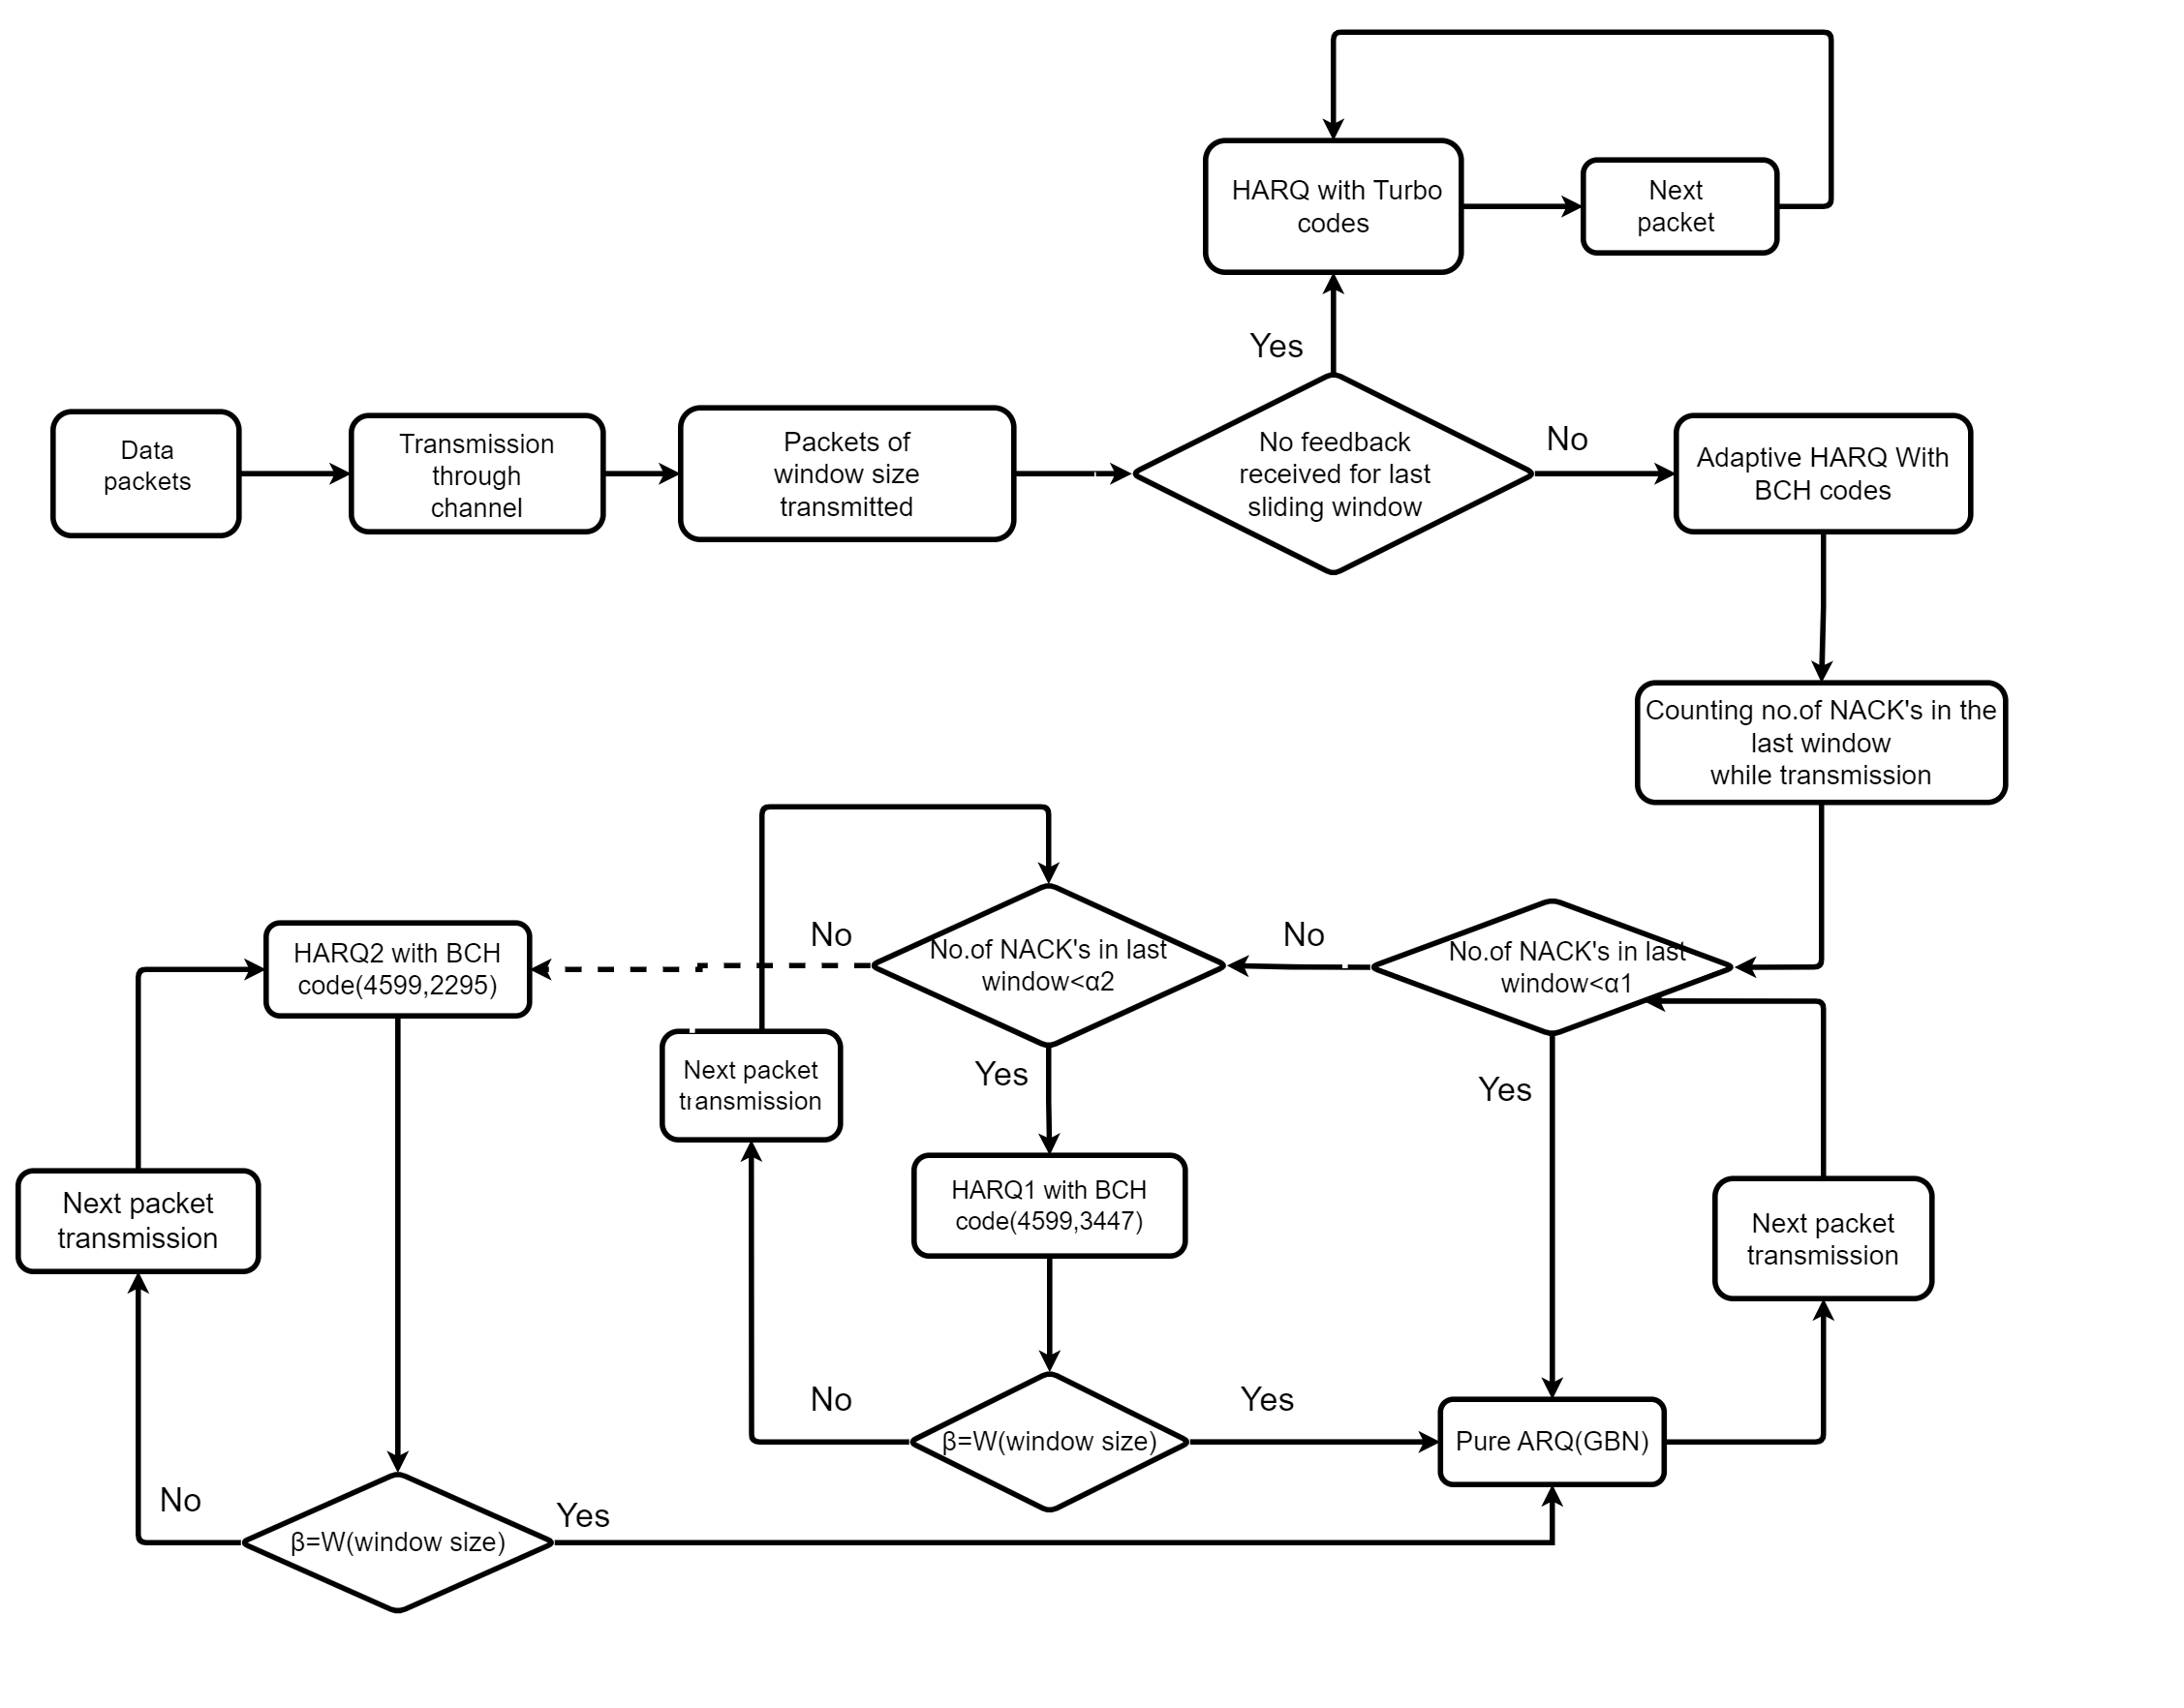
\includegraphics[width=\textwidth]{SWITCH.png}
    \caption{Illustration of the dynamic switching between different HARQ schemes}
    \label{fig:5}
\end{figure}

The main parameter used to switch between the schemes is the number of NACKs. If the count of NACKs crosses the threshold $\alpha_1$, the scheme switches from ARQ to HARQ1, as shown in Figure \ref{fig:5}. To calculate $\alpha_1$, first equate the throughput of ARQ with the throughput of HARQ1.

\begin{equation}
\frac{1 - P_e}{1 + S \cdot P_e} \cdot \frac{N \cdot b - CRC}{N \cdot b} = \frac{K}{N} \times \frac{1 - \sum_{i=t+1}^{N} \binom{N}{i} P_s^i (1-P_s)^{N-i}}{1 + S \cdot \sum_{i=t+1}^{N} \binom{N}{i} P_s^i (1-P_s)^{N-i}}
\label{14}
\end{equation}

Replace ${P}_e$ with Eq. \ref{7} and ${P}_s$ with the equation in the Eq. \ref{14}.

The unknown variable ${P}_b$ can be calculated by solving the above equality. By substituting this ${P}_b$ value in Eq. \ref{7}, ${P}_e$  can be derived and the threshold $\alpha_1$ is given by

\begin{equation}
    \alpha_1 = P_e \cdot W
\end{equation} 

where W denotes window size.
 
To calculate the threshold $\alpha_2$ that determines when to switch from HARQ1 to HARQ2,  equate the throughput expressions of both HARQ schemes.
 
\begin{equation}
\frac{K1}{N} \times \frac{1 - \sum_{i=t+1}^{N} \binom{N}{i} P_s^i (1-P_s)^{N-i}}{1 + S \cdot \sum_{i=t+1}^{N} \binom{N}{i} P_s^i (1-P_s)^{N-i}} \nonumber \\
= \frac{K2}{N} \times \frac{1 - \sum_{i=t+1}^{N} \binom{N}{i} P_s^i (1-P_s)^{N-i}}{1 + S \cdot \sum_{i=t+1}^{N} \binom{N}{i} P_s^i (1-P_s)^{N-i}} \label{eq:combined2}
\end{equation}

From this equality, the unknown variable $P_s$ can be calculated. Then the threshold $\alpha_2$ is given by

\begin{equation}
    \alpha_2 = P_s \cdot W
\end{equation}

On the other hand, when no error is detected in the last sliding window, a new kind of acknowledgment ACK+ is sent to the transmitter. Then the scheme switches back from HARQ1 or HARQ2 to ARQ as the signal quality is exceptionally good, as shown in Figure \ref{fig:5}. When channel conditions are favorable, this transition back to pure ARQ significantly reduces unnecessary costs. This threshold for the number of acknowledgments is denoted by $\beta$. Where $\beta$=W indicates that the W acknowledgments are sent consecutively. The detailed flow of the switching scheme is shown in Figure \ref{fig:5}. In the observed scenario, adaptive HARQ with BCH codes shows negligible throughput under SNR conditions ranging from 0 to 3.47 dB. However, when HARQ with turbo codes is used, a substantial improvement in throughput can be observed at very low SNR values in Figure \ref{fig:6}; this suggests that turbo codes could effectively enhance throughput in this specific range.

\subsection{Detailed mechanism of HARQ with Turbo Codes} \label{s3.4}

This subsection explains the mechanism of HARQ with turbo codes in the D-HARQ model. Initially, the packet undergoes a series of encoding phases to enhance error correction capabilities. As shown in Figure \ref{fig:15}, the first phase, known as Bit Splitting, prepares the input bitstream for parallel processing. This is followed by Constituent Encoding 1, where the first half of the bitstream is convolutionally encoded, introducing redundancy that serves as the foundation for error correction. To further improve the ability to correct errors, the bitstream undergoes interleaving, ensuring a more uniform distribution of potential errors across the bitstream. The process continues with Constituent Encoding 2, adding an additional layer of redundancy through a second convolutional encoder. Finally, Rate Matching is applied to adjust the encoded bitstream according to the transmission channel's specific bandwidth and error characteristics. Upon completion of the encoding stages, the data are ready for modulation onto a carrier signal and transmitted across the communication channel, where it is prone to noise and interference. At the receiving end, the Reception and Signal Demodulation stage takes over, where the transmitted signal is captured and demodulated to retrieve the encoded data bitstream.

\begin{figure}[H]
    \centering
    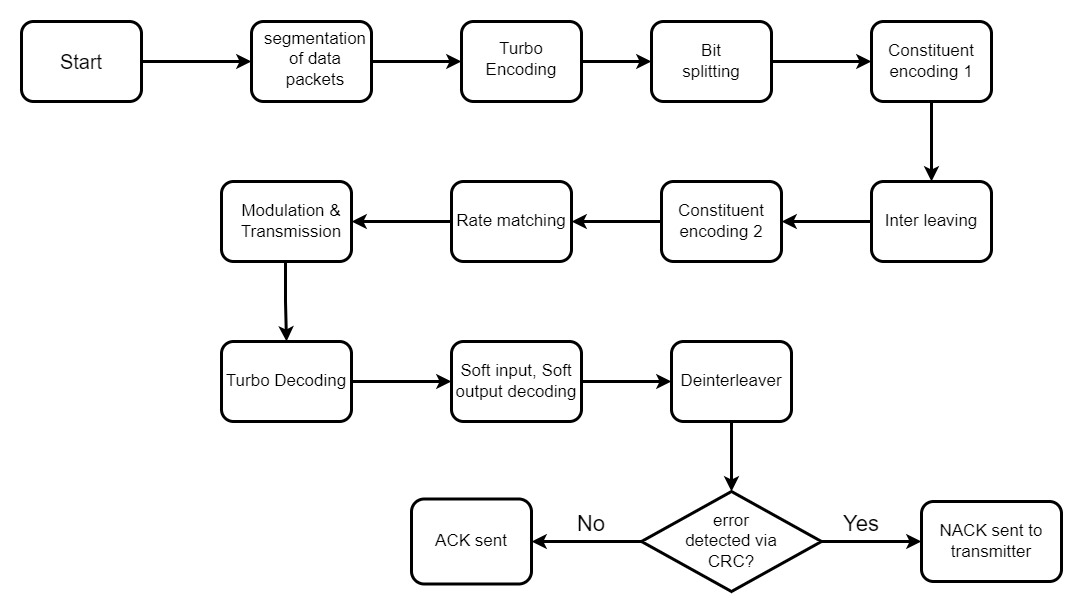
\includegraphics[width=\textwidth]{turbo_flow.jpg}
    \caption{HARQ with Turbo codes}
    \label{fig:15}
\end{figure}

The turbo decoding process begins with Soft-input Soft-output Decoding Iteration 1 as depicted in Figure \ref{fig:15}. This phase marks the initial attempt to decode the received signal, using soft decision inputs to produce soft decision outputs. These outputs include probability metrics that indicate the accuracy of each bit, significantly enhancing the decoding process's effectiveness. The Deinterleaver reorders bits between decoding iterations. Subsequent iterations of the decoding are required to refine the accuracy of the data. After decoding, error detection is conducted through the Cyclic Redundancy Check (CRC), prompting a NACK for retransmission if errors are detected or an acknowledgment (ACK) for error-free data, signaling successful reception. 

\subsection{SNR estimation algorithm } \label{s3.1}

This subsection provides a detailed explanation of the SNR estimation algorithm, which is a crucial requirement for the selective soft-combining process. The Error Vector Magnitude (EVM) SNR estimation Algorithm \ref{alg:snr_estimation} has been used to improve the accuracy and scope of SNR estimation. This advancement comes in response to the limitations of current methodologies, which struggle with accurately estimating low SNRs. Initially, the mean and variance of the signal samples $|y_n|$ at time instants n = 1, 2, ..., L after downsampling are calculated as below in Eq. \ref{1}, Eq. \ref{2}.

\begin{equation}\label{1} 
\text{mean} = \frac{1}{L} \sum_{n=1}^{L} |y_n|
\end{equation}

\begin{equation}\label{2} 
\text{var} = \frac{1}{L} \sum_{n=1}^{L}( |y_n| -\text{mean})^2
\end{equation}

SNR is calculated from Eq. \ref{3} using these results.

\begin{equation}\label{3} SNR = 10 \times \log\left(\frac{|\text{mean}|^2}{2 \times \text{var}}\right) \end{equation}

When the estimated value is less than 10dB, the intermediate z value temporarily stores this SNR. 

\begin{equation} 
    z = SNR
\end{equation}

the new SNR' is estimated by using the z value.

\begin{equation}
\text{SNR' } = \sqrt{ (z - 2.5) \times 39.2 } - 7
\end{equation}

When the SNR is below 10 dB, the SNR' provides an accurate estimate; otherwise, the SNR is considered acceptable. This algorithm has a higher estimation accuracy and less deviation in a larger range between -10 to 30 dB. The complexity of the algorithm is low as it uses only the mean and variance of the data.

\begin{algorithm}
    \caption{SNR Estimation Algorithm \cite{r20}}
    % \rule{\linewidth}{0.5pt}\\
    \rule{\linewidth}{0.5pt}\\
    \label{alg:snr_estimation}
    \begin{algorithmic}[1]
        \State \textbf{Input:} Received signal samples $y_n$, number of samples $L$
        \State \textbf{Output:} Estimated SNR
        \State Compute mean and variance:
        \State \quad $\text{mean} \gets \frac{1}{L} \sum_{n=1}^{L} |y_n|$
        \State \quad $\text{var} \gets \frac{1}{L} \sum_{n=1}^{L} (|y_n| - \text{mean})^2$
        \State Compute SNR:
        \State \quad $\text{SNR} \gets 10 \times \log_{10}\left(\frac{|\text{mean}|^2}{2 \times \text{var}}\right)$
        \If{$\text{SNR} < 10$ dB}
            \State Compute intermediate value:
            \State \quad $z \gets \text{SNR}$
            \State Compute new SNR':
            \State \quad $\text{SNR'} \gets \sqrt{(z - 2.5) \times 39.2} - 7$
            \State \Return $\text{SNR'}$
        \Else
            \State \Return $\text{SNR}$
        \EndIf
    \end{algorithmic}
\end{algorithm}

\subsection{Decision Making for Soft Combining at Receiver End} \label{s3.5}

This subsection explains how the receiver decides whether to perform soft combining or not based on the current channel conditions. At the receiver end, the choice of soft combining is made by estimating the SNR value of the received signal using the EVM algorithm as discussed in Section \ref{s3.1}. This algorithm is advantageous because it can estimate accurate SNR values even at very low SNR conditions. Since calculating the SNR for every signal can be complex at the receiver end, calculating at regular intervals reduces the overhead.

Soft combining is a technique that involves combining the retransmitted data with previously received erroneous blocks to enhance decoding accuracy. However, when the channel conditions are perfect, the benefits of soft combining might be limited. It can be observed in Section \ref{s4}. This is because the individual received signals are already of high quality. Therefore, it might be more efficient to avoid soft combining to save computational resources and reduce complexity. Thus, soft combining should be done selectively by estimating the channel conditions through SNR.

\begin{figure}[H]
    \centering
    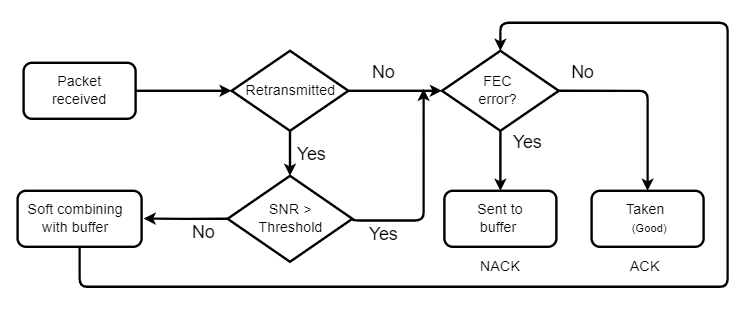
\includegraphics[width=0.8\textwidth]{sf.png}
    \caption{ Illustration of the decision-making for soft combining at the receiver end}
    \label{fig:8}
\end{figure}

Upon receiving a packet, as shown in Figure \ref{fig:8}, the first step is to determine whether it is an original transmission or a retransmission. If the packet is not retransmitted, it is sent directly to the error detection module. If no errors are detected, it is accepted directly. However, if errors are identified, it is forwarded to the buffer and NACK is sent to the transmitter to request the packet to be retransmitted. 

However, if the packet is identified as retransmitted, a decision must be made about whether to apply soft combining. This decision is based on the estimated SNR calculated from the EVM algorithm. If the SNR exceeds the predetermined threshold, it signifies a strong signal quality, suggesting that the packet is likely error-free. In such scenarios, merging this packet with previously errored packets in the buffer could degrade performance. Consequently, the packet is directly sent to the error detection module without undergoing soft combining, as shown in Figure \ref{fig:8}. In contrast, soft combining is employed if the SNR does not meet the threshold, indicating a weaker signal. This strategy improves throughput and reduces the required retransmissions by utilizing the cumulative information from multiple receptions of the same packet.

\section{Results and Anlaysis} \label{s4}

Simulations of D-HARQ were conducted within the Land Mobile and Satellite (LMS) channel using MATLAB and Python, focusing on rural and suburban environments. LMS channel facilitates communication between land-based mobile stations and satellites, allowing wide geographic coverage for services such as GPS, satellite phones, and remote sensing in remote or rural areas. Under these conditions, the energy loss in the Line-of-Sight (LOS) wave is comparatively insignificant. LOS is an unobstructed path between transmitter and receiver, offering reliable communication with minimal signal attenuation, crucial for applications like microwave links and satellite communication. Consequently, signal propagation in this context follows a log-normal distribution with the probability density function (PDF), as detailed below:

\begin{equation}
f(x) = \frac{e^{-\left(\frac{(\ln x)^2}{2\sigma^2}\right)}}{x\sigma\sqrt{2\pi}}
\end{equation} 

For x $>$ 0, where x is the random variable representing the signal strength and $\sigma$ is the distribution of additive white Gaussian (AWGN) noise.

Table \ref{tab:2}  details the number of information bits and associated redundancy bits, such as CRC for ARQ and error-correcting bits for HARQ1 and HARQ2. This information illustrates the error correction capabilities of each scheme in communication systems. Furthermore, Table \ref{tab:1} illustrates the simulation environment.

\begin{table}[!htbp]
\caption{Number of information and redundancy bits for various schemes}
\label{tab:2}
\centering
\small
\renewcommand{\arraystretch}{1.5} 
\begin{tabularx}{\columnwidth}{|>{\raggedright\arraybackslash}X|>{\raggedright\arraybackslash}X|>{\raggedright\arraybackslash}X|} \hline
    \textbf{Scheme} & \textbf{Information bits} & \textbf{Redundancy bits} \\ \hline
    ARQ & 4567 & 32 (CRC) \\ \hline
    HARQ1 with BCH codes & 3447 & 1152 \\ \hline
    HARQ2 with BCH codes & 2295 & 2304 \\ \hline
\end{tabularx}
\end{table}

\begin{table}[!htbp]
\caption{Simulation environment and parameters}
\label{tab:1}
\centering
\small
\renewcommand{\arraystretch}{1.5}
\setlength\tabcolsep{4pt} 
\begin{tabularx}{\columnwidth}{|>{\raggedright\arraybackslash}X|>{\raggedright\arraybackslash}X|} \hline
    \textbf{Parameters} & \textbf{Values} \\ \hline
    Channel model & Land, Mobile, and Satellite \\ \hline
    Channel conditions & Rural and Suburban \\ \hline
    ARQ Scheme & ARQ, HARQ1, HARQ2  \\ \hline
    No. of symbols in each block/packet & 511 \\ \hline
    No. of bits per symbol &  9  \\ \hline
    Delay & 5 $\times$ No. of information symbols \\ \hline
    Noise & White Gaussian (AWGN) noise  \\ \hline
    Simulation output & Matlab with Python codes  \\ \hline
    Simulated SNR range & 0-18 dB \\ \hline  
\end{tabularx}
\vspace{0.1in}
\end{table}

\begin{figure}[H]
    \centering
    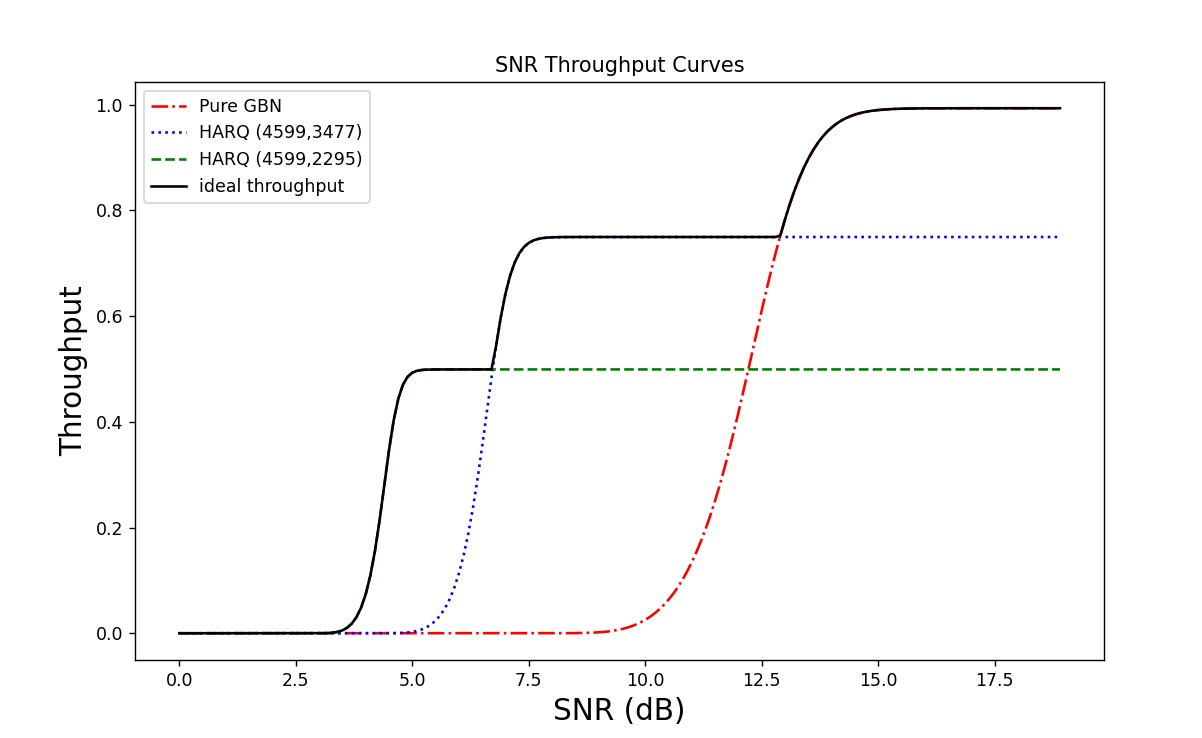
\includegraphics[width=\textwidth]{bch.jpg}
    \caption{Transitions between various HARQ and ARQ schemes}
    \label{fig:7}
\end{figure}

Figure \ref{fig:7} illustrates a graph of a D-HARQ model, highlighting the thresholds for transitioning between different modes, which have been established through a trial-and-error methodology. The simulations are performed for various sets of thresholds. Ultimately, the graph is almost aligned with the ideal curve for $\alpha1$ = 10, $\alpha2$ = $\beta$ = W= 64. Here, the throughput of the ideal curve at a given SNR is expressed as

\begin{equation}
    \eta_{\text{ideal}} = \max(\eta_{\text{ARQ}}, \eta_{\text{HARQ1}}, \eta_{\text{HARQ2}})
\end{equation}

Figure \ref{fig:7} demonstrates the performance benefits of implementing an adaptive HARQ strategy within the SNR range of 3.47 to 9 dB, compared to a traditional GBN approach. Adopting the D-HARQ method in this specific SNR interval substantially increases throughput, achieving a gain of approximately $2.16\times 10^{16}$ times. Moreover, Figure \ref{fig:7} highlights the enhanced throughput achieved by utilizing two different states of HARQ, each configured with BCH codes of varying code rates. A notable throughput enhancement of 31.67\% is observed when transitioning from HARQ state 2 to HARQ state 1 within the SNR range of 6.68 to 12.89 dB. The D-HARQ model recommends transitioning from HARQ back to ARQ at higher SNR values, a strategy that is convincingly supported by the simulation curve. This curve demonstrates the necessity for such a switch, highlighting a significant improvement of about 28.5\% in throughput above 12.89 dB.

The main drawback observed in Figure \ref{fig:7} is a negligible throughput that is close to zero in the 0 to 3.47dB range. This D-HARQ model successfully avoids this by adapting HARQ with turbo codes in this range.

\begin{figure}[H]
    \centering
    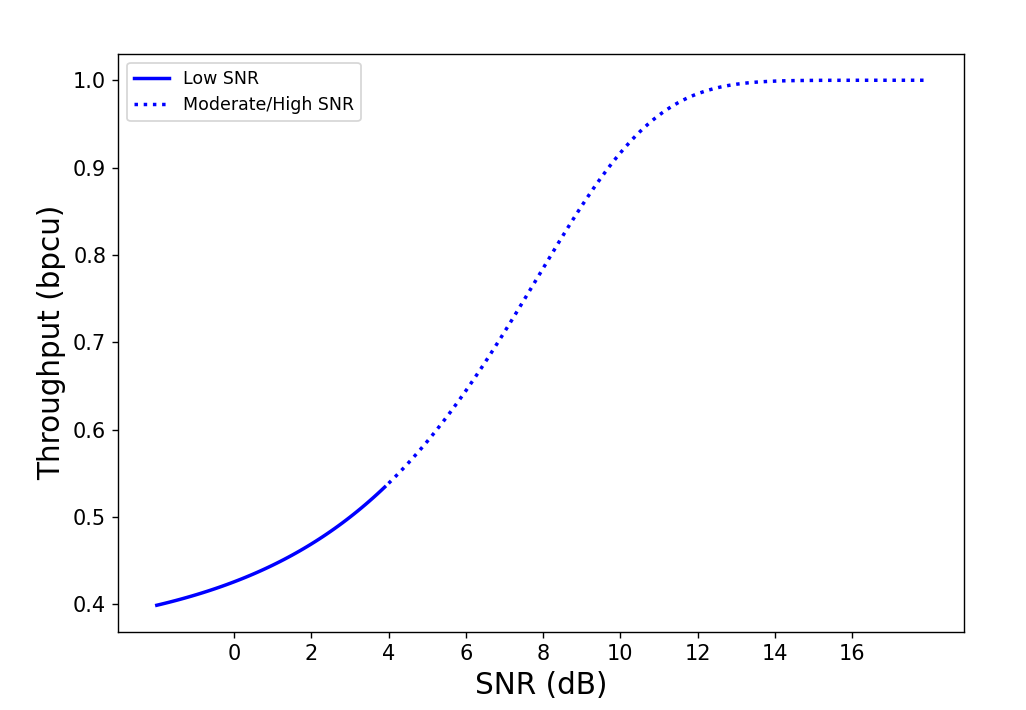
\includegraphics[width=\textwidth]{turbo_code.png}
    \caption{Estimated Throughput vs SNR for HARQ with Turbo codes (code rate = 1/3)}
    \label{fig:6}
\end{figure}

Figure \ref{fig:6} shows considerable throughput even at low SNR values, which is an improvement in throughput from 0 to 0.467 bpcu by adapting turbo codes. In Figure \ref{fig:6}, the feasibility of using turbo codes in all SNR ranges may be questioned. Implementing Turbo Codes, while offering superior error correction capabilities, particularly in environments with a high SNR, presents a more complex challenge than BCH codes due to several key factors. First, the architecture of Turbo Codes involves an intricate iterative decoding process, which relies on passing information back and forth between two or more constituent decoders. This interplay requires a sophisticated algorithm to effectively converge on the correct decoding, significantly complicating the implementation compared to the straightforward algebraic decoding methods used for BCH codes.

As explained in Section \ref{s2}, soft combining is beneficial as combining the retransmitted packet with the error packets in the buffer improves its decoding capability, thus reducing the need for retransmissions. However, at a very high SNR, the idea of soft combining does not contribute much to throughput improvement. Thus, in these scenarios, there is no need to adapt such schemes, thus optimizing the complexity and minimizing the usage of resources.

\begin{figure}[H]
    \centering
    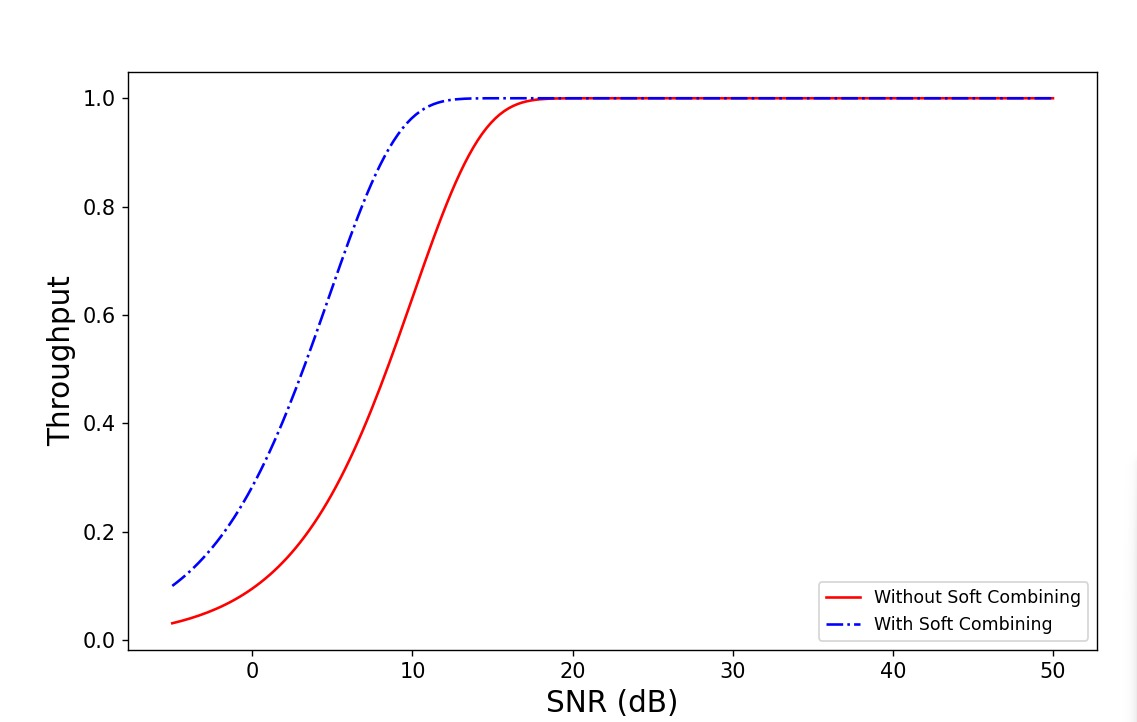
\includegraphics[width=\textwidth]{soft_combining.jpg}
    \caption{Performance comparison with and without Soft combing}
    \label{fig:9}
\end{figure}

Figure \ref{fig:9} compares throughput with and without soft combining at all SNR values ranging from 0 to 50 dB. Thus, the threshold to selectively soft combine is 17.46 dB; therefore, SNR above this threshold indicates that the channel quality is good enough to omit soft combining.

\section{Conclusion and Future works} \label{s5}

This paper introduced D-HARQ, an SNR responsive scheme that switches between ARQ and HARQ using BCH and turbo coding. In addition, it is integrated with the selective soft combining method for improved performance. The strategic utilization of turbo codes under very low SNR conditions and BCH codes in other scenarios strikes an optimal balance between cost-effectiveness and reliability. As soft combining is selectively avoided under good channel conditions, the associated complexity overhead is minimized, improving performance and maximizing throughput. The effectiveness of this paper's proposal is validated through simulation results using turbo coding and selective soft combining. These results demonstrate a significant improvement in throughput while reducing complexity at every level of data transmission. Future work could involve initiating simulations and using machine learning to determine accurate thresholds.

\section*{\textbf{Statements \& Declarations}}

\subsection*{Competing Interests}
I have no conflicts of interest to disclose. No financial conflicts with any author
or agencies.

\subsection*{Funding}
The authors declare that no funds, grants, or other support was received during the preparation of this manuscript.

\subsection*{Author Contributions}
Material preparation and analysis of the materials was done by me only.

\subsection*{Data availability statements (DAS)}
As our own

\subsection*{Research Involving Human and /or Animals}
As our own

\subsection*{Informed Consent}
Not applicable


\bibliography{reference}

\end{document}


